\documentclass[a4paper,11pt,openright,openbib]{article}
\usepackage[portuges]{babel}
\usepackage[T1]{fontenc}
\usepackage{ae}
\usepackage[utf8]{inputenc}
\usepackage[pdftex]{graphicx}
\usepackage{url}
\usepackage{listings}
\usepackage{verbatim}
\usepackage{enumerate}
\usepackage{epstopdf}
\usepackage[a4paper, pdftex, bookmarks, colorlinks, linkcolor=black, urlcolor=blue]{hyperref} 
\usepackage[a4paper,left=2.5cm,right=2.5cm,top=3.5cm,bottom=3.5cm]{geometry}
\usepackage{colortbl}
\usepackage[margin=10pt,font=small,labelfont=bf]{caption}
\usepackage{mdwlist}


\setlength{\parindent}{0cm}
\setlength{\parskip}{2pt}




\title{
	\large{\includegraphics[width=0.3\textwidth]{../../report-template/UM.jpg}} \\
	\large{Universidade do Minho}  \\
	\large{Mestrado em Engenharia Informática}  \\
	\large{Engenharia de Linguagens}  \\
	\large{Projecto Integrado - Grupo 1}  \\	
	\large{\textbf{1ª Avaliação Intermédia}} \\
	\large{Ano Letivo de 2012/2013} \\
	\date{\today}
}

\author{	
	\begin{tabular}[t]{c c}      
        pg22820 - \textbf{António Silva} \\        
	pg22781 - \textbf{Rui Brito} \\   				
	\\ 
	\end{tabular}
}

\begin{document}

\maketitle


\pagestyle{headings}
\pagenumbering{arabic}
\newpage
\tableofcontents
\newpage

\section{Introdução}
O projecto consiste no desenvolvimento de um sistema de informação que permita gerir os dados curriculares de um docente universitário.\\
Essa informação a recolher, armazenar e publicar inclui, além da identificação completa do docente, dados sobre a formação, as várias actividades académicas desenvolvidas e resultados atingidos.\\
Neste primeira fase eram pedidos o planeamento, a modelação (Diagrama de classes, Esquema de Base de Dados, Use Cases...), uma gramática e respectivo processador para uma linguagem de informação e formação, e ainda uma esquema de uma linguagem de anotação para as actividades desenvolvidas.


\section{Planeamento}

\section{Modelação}

\subsection{Diagrama de Classes}
\begin{figure}[!ht]
\centering
\includegraphics[scale=.4]{Diagrama_Classes.jpg}
\caption{Diagrama de Classes}
\label{fig:diagramadeclasses}
\end{figure}
O Diagrama de Classes, presente na figura \ref{fig:diagramadeclasses} inicialmente desenvolvido estava consideravelmente mais pobre e foi enriquecido também à medida que fomos avançando no projecto. Foi também um enorme ponto de partida para a criação da Base de Dados. A única parte ainda bastante subdesenvolvida é a dos resultados pelo facto de ainda não termos avançado muito nessa questão e ter ficado somente aquilo que retirámos das primeiras leituras, quer do enunciado, quer de exemplos facultados ou encontrados.
\subsection{Use Cases}
\begin{figure}[!ht]
\centering
\includegraphics[scale=.6]{Use_Cases.jpg}
\caption{Use Cases}
\label{fig:usecases}
\end{figure}
Os \emph{Uses Cases} na figura \ref{fig:usecases} referem-se essencialmente a tarefas possíveis de serem feitas, quer pelo Gestor, quer pelo Académico (na maioria dos casos o académico será o docente).\\
Cada \emph{Use Case} possui uma descrição textual que nos permitiu já ponderar um pouco sobre como irá o sistema responder ao utilizador e interagir com outros sistemas. Podemos ver dois exemplos da descrição textual dos uses cases na figura \ref{fig:uc_consultcv} e \ref{fig:uc_providecvinfo}
\begin{figure}[!ht]
\centering
\includegraphics[scale=1]{uc_consult_cv.jpg}
\caption{Use Case - Consult CV}
\label{fig:uc_consultcv}
\end{figure}
\begin{figure}[!ht]
\centering
\includegraphics[scale=.9]{uc_provide_cv_info.jpg}
\caption{Use Case - Provide CV\rq{}s info}
\label{fig:uc_providecvinfo}
\end{figure}

\subsection{Base de Dados}
\begin{figure}[!ht]
\centering
\includegraphics[scale=1]{bd.eps}
\caption{Base de Dados}
\label{fig:basededados}
\end{figure}
A estrutura da base de dados (figura \ref{fig:basededados}) foi pensada de forma a permitir armazenar, como é óbvio, os dados que foram analisados por exemplo no diagrama de classes. Os seus relacionamentos foram facilmente idealizados.


\section{Linguagem formal para Identificação e Formação}
\subsection{Gramática}
A Gramática para a linguagem de identificação e formação foi facilmente criada, recorrendo ao que já tínhamos analisado para o diagrama de classes. No entanto, permitiu-nos também enriquecer mais o diagrama de classes, pois ao irmos escrevendo a gramática lembramo-nos de coisas que nos poderiam fazer falta.\\
Apesar de tudo não refinámos ainda muito certos campos como o email e o web porque são coisas definidas por normas externas, que queríamos tentar seguir e adaptar à gramática desenvolvida no AntLR.\\
Também aqui decidimos fazer, que permita futuras actualizações em implicar uma completa reestruturação da gramática. Uma delas foi aquilo a que nos chamamos \emph{Special ID} (SPID), por exemplo para valores como o País. Isto porque o País é um cujo os valores podem ser normalizados de modo a que não existam dois países iguais com nomes diferentes, e poderá permitir mais para a frente se acharmos conveniente criar mais uma relação na Base de Dados, de modo a reduzir o espaço ocupado, por exemplo pelas nacionalidades.
\begin{verbatim}
SPID
	:	('A'..'Z')('a'..'z')* (' '('A'..'Z')('a'..'z')*)*
	;
\end{verbatim}
\subsection{Processador}
Quando discutimos o nosso processador, foi ponto assente, que queríamos evitar a repetição de código, assim sendo tentamos passar grande parte da responsabilidade para o ficheiro \emph{info\_import.php}, que seria um \emph{template}. Assim grande parte das coisas geradas pelo Parser seriam simplesmente valores etiquetados que ele saberia onde colocar.\\
Infelizmente não tivemos muito tempo para implementar a detecção de erros semânticos e assim, apesar de ele já detectar erros, como a data de início ser superior às de fim, apenas mostra essa mensagem mas continua o processamento.\\
Também neste momento o formulário para importação do documento é bastante reduzido, e serve simplesmente para indicar o ficheiro em questão.
\begin{verbatim}
<html>
	<head></head>
	<body>
	<form method=\"post\" action=\"info_import.php\" enctype=\"multipart/form-data\">
            <fieldset>
                <legend>Info e Form:</legend> 
			<input type='file' name='ficheiro'/>
	    </fieldset>
	    <input type=\"submit\" name=\"Enviar\"/>
	</form>
	</body>
</html>
\end{verbatim}
O código de execução do \emph{parser} e leitura dos resultados também não é muito complexa. No entanto permite que estejam vários utilizadores simultâneos a executar a aplicação web, sem existir nenhum tipo de conflitos já que o \emph{stdout} é redireccionado para a leitura do php através de um \emph{handler}.
\begin{verbatim}
$f = (popen('java -jar AntLRParser.jar "'.$_FILES['ficheiro']['tmp_name'].'"', "r"));

$valor = "";
while (!feof($f)) {$valor .= fread($f, 60);}
\end{verbatim}
Depois as inserções são feitas na Base de Dados MySQL recorrendo à classe PDO do php.
\subsection{Exemplo de Input}
Aqui está um exemplo de \emph{input} válido para a gramática desenvolvida.
\begin{verbatim}
@info {
	Name: "xpto"
	Nationalities: [Portuguese,Canadian]
	PersonalContacts: [
					Phone: "252000000" , 
					Email: xpto@st.pt
					]
	Birthdate: 13/05/2001
	Gender: M
	NativeLang: [Portuguese,English]
	Web: http://xpto.com
}
@form {
	Begin: 01/01/2008
	End: 01/02/2012
	Institution: 
		Name: "Universidade do Minho"
		Address: "Gualtar Braga"
		Country: Portugal
		Type: Public University
	Degree: BSc "Engenharia Informática"
	Result: 20
}
\end{verbatim}
\section{Linguagem de anotação para descrição das Actividades}
O \emph{Schema} (na figura \ref{fig:cv_activities}) desenvolvido para a descrição de actividades, teve também por modelo o que já tínhamos definido para a Base de Dados, para tentar equilibrar os dados que poderiam ser guardados e os que seriam enviados.\\
Um facto bastante relevante é permitir que uma actividade esteja relacionada com mais que um utilizador, podendo descrevê-lo como utilizador do sistema, ou não utilizador (e indicando somente o seu nome).
\begin{figure}[!ht]
\centering
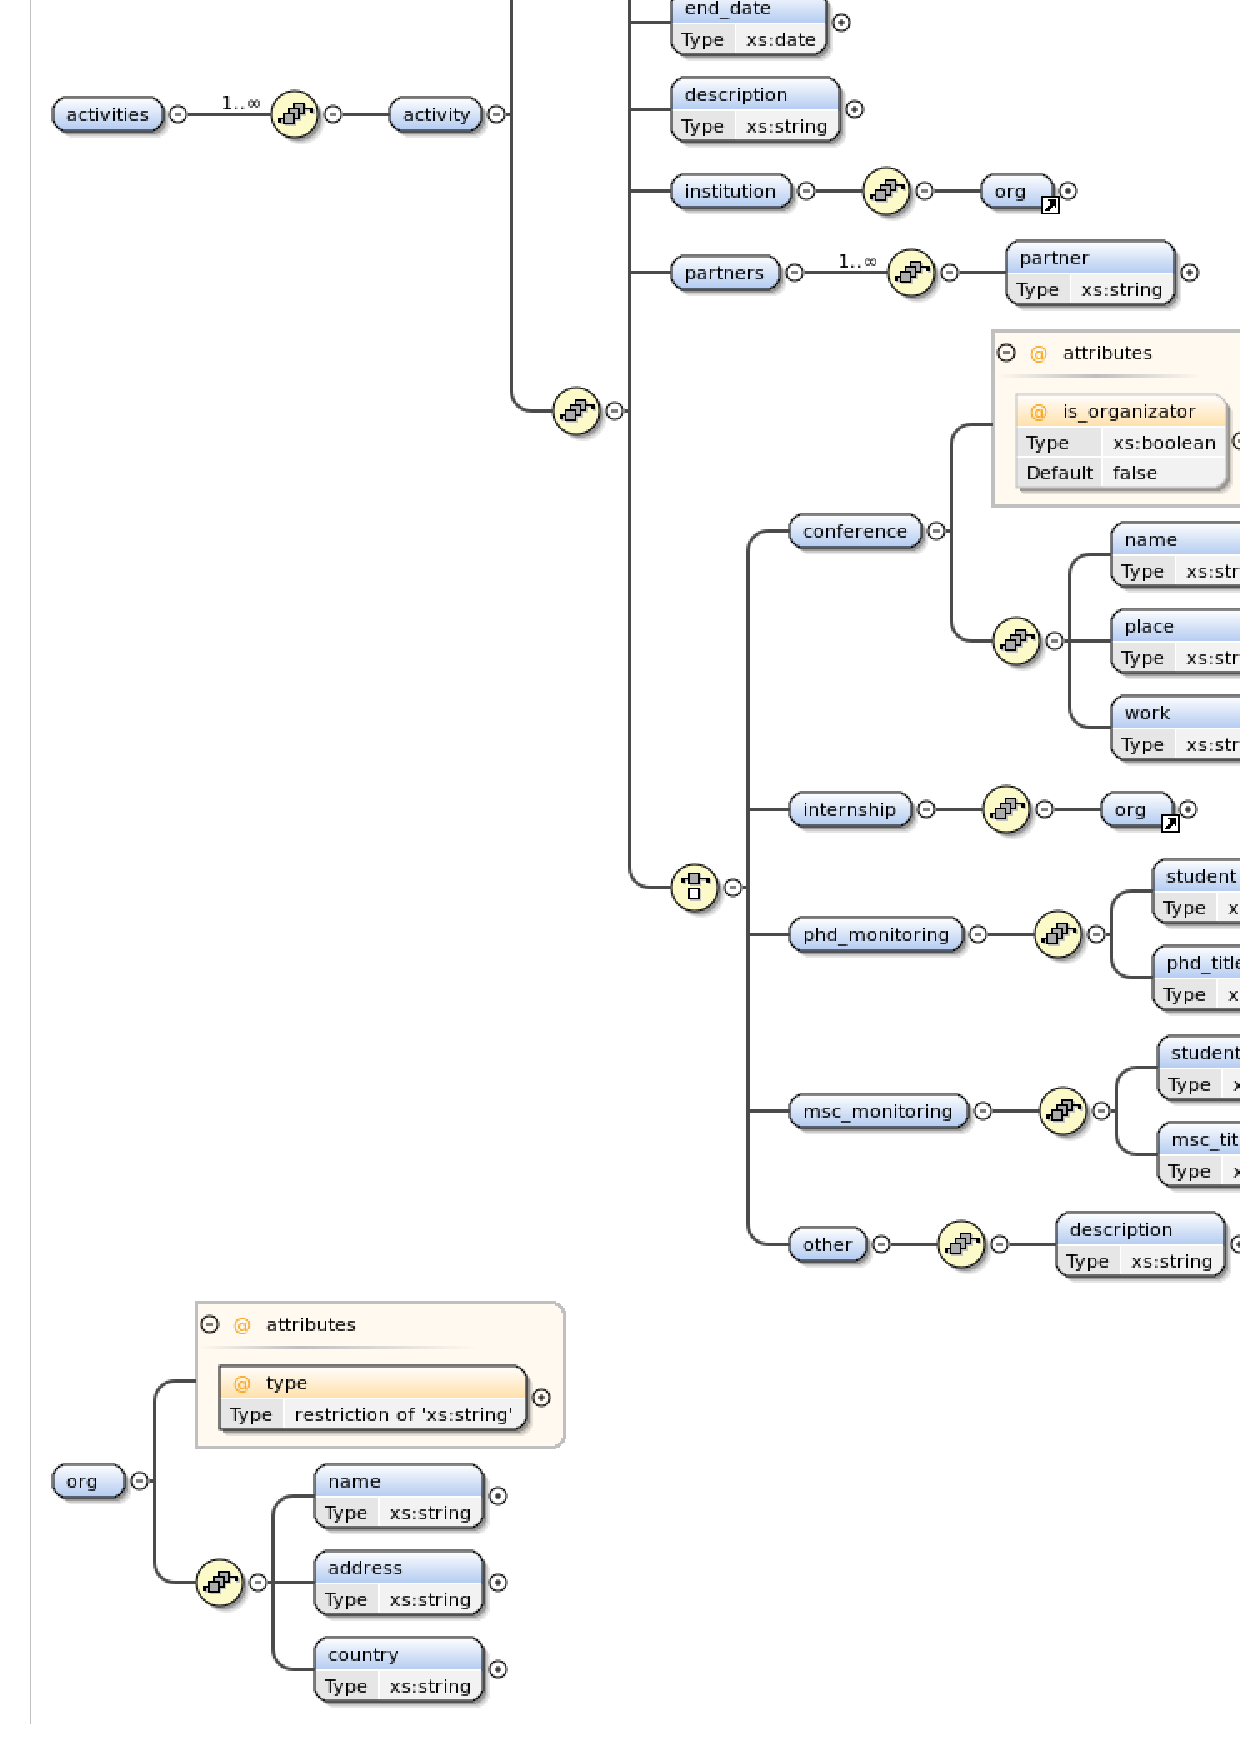
\includegraphics[scale=0.75]{cv_activities_schema.png}
\caption{Schema da linguagem}
\label{fig:cv_activities}
\end{figure}

\section{Conclusão}
O objectivo desta primeira avaliação do Projecto Integrado, é garantir que o mesmo segue já a um bom ritmo, servindo também já como um suporte para o desenvolvimento futuro, na medida em que será uma base sobre a qual podemos continuar a construir já mais cientes dos caminhos correctos que escolhemos e daqueles que não estavam assim tão correctos, ao ser mostrado à equipa docente os resultados obtidos até à data.
\end{document}